%%%%%%%%%%%%%%%%%%%%%%%%%%%%%%%%%%%%%%%%%
%	
%	Clusters particionais com dados numéricos
% 	The Elbow Method

%%%%%%%%%%%%%%%%%%%%%%%%%%%%%%%%%%%%%%%%%

%----------------------------------------------------------------------------------------
%	PACKAGES AND OTHER DOCUMENT CONFIGURATIONS
%----------------------------------------------------------------------------------------

\documentclass[12pt, a4paper, oneside]{scrreport}
\usepackage[T1]{fontenc}
\usepackage{wrapfig}
\usepackage[portuguese]{babel} 
\usepackage{graphicx}
\usepackage{amsmath}
\usepackage{amsfonts}
\usepackage{multicol}
\usepackage{setspace}
\usepackage[hyphens]{url}
\usepackage{utopia}
\usepackage{hyperref}
\usepackage[dvipsnames]{xcolor}
%\usepackage{fancyhdr}
\usepackage{libertine}
\usepackage{blindtext}
\usepackage[plainfootsepline]{scrlayer-scrpage}
\usepackage{listings}
\usepackage{caption}
\usepackage{subcaption}
\usepackage{enumitem}
\usepackage{animate}
\usepackage{algorithm}
\usepackage[noend]{algpseudocode}

%-------------------------------------------------------------------------------
%	SPECIFIC CONFIGURATIONS 
%---------------------------------------------------------------------
 
\DeclareMathOperator{\dist}{dist} 
 
%Algpseucode

\renewcommand{\algorithmicrepeat}{\textbf{repita}}
 \renewcommand{\algorithmicuntil}{\textbf{at\'{e}}}
 \renewcommand{\algorithmicfor}{\textbf{para}}
  \renewcommand{\algorithmicdo}{\textbf{faz}}
 \renewcommand{\algorithmicend}{\textbf{fim}}
% \renewcommand{\algorithmicendfor}{\algorithmicend\ \algorithmicfor}
 \renewcommand{\algorithmicprocedure}{\textbf{procedimento}}

%MULTICOL

\setlength{\columnsep}{1cm}

%INCLUDEGRAPHICS

\graphicspath{{Figures/}} %Pasta de input de imagens, gráficos, ...

%HYPERREF
\hypersetup{
	colorlinks=true,
	linkcolor=black,
	urlcolor=black,
    urlbordercolor=black,
    linkbordercolor=white,
    pdfborderstyle={/S/U/W 1},
    pdftitle={The Elbow Method},
    pdfpagemode=FullScreen
}

\makeatletter
\Hy@AtBeginDocument{%
  \def\@pdfborder{0 0 1}% Overrides border definition set with colorlinks=true
  \def\@pdfborderstyle{/S/U/W 1}% Overrides border style set with colorlinks=true
                                % Hyperlink border style will be underline of width 1pt
}
\makeatother

%CAPTIONS

\DeclareCaptionType{myequation}[][Lista de Equações]
\captionsetup[myequation]{labelformat=empty}


%-------------------------------------------------------------------------------
%	Colors
%-------------------------------------------------------------------------------

\definecolor{uminho}{RGB}{125,58,64}


%-------------------------------------------------------------------------------
%	Chapter Style
%-------------------------------------------------------------------------------
\RedeclareSectionCommand[
  beforeskip=1sp minus 1sp,
  font=\Huge\fontfamily{put}\color{white}
]{chapter}

\renewcommand\chapterformat{%
  \makebox[0pt][r]{\Huge{\thechapter}\enskip
    \textcolor{white}{\smash{\rule[-0.5\dp\strutbox]{3pt}{1cm}}}%
}}

\newlength\chapterleftmargin
\newcommand\chaptervmargin{1.5em}

\makeatletter
\renewcommand\chapterlinesformat[3]{%
  \vspace*{\dimexpr-1in-\headsep-\headheight-\topmargin-1ex}%
  \Ifthispageodd
    {\setlength\chapterleftmargin{\dimexpr1in+\hoffset+\oddsidemargin\relax}}
    {\setlength\chapterleftmargin{\dimexpr\paperwidth-\textwidth-1in-\hoffset-\oddsidemargin\relax}}
    \hspace*{-\chapterleftmargin}%
    \makebox[0pt][l]{%
      \colorbox{uminho}{%
        \parbox[t][\dimexpr\totalheight+\chaptervmargin*2\relax][c]{\dimexpr\paperwidth-2\fboxsep\relax}{%
          \makebox[\dimexpr\chapterleftmargin-\fboxsep\relax][r]{#2}%
          \Ifstr{#2}{}
            {\parbox[t]{\textwidth}{\raggedchapter#3}}
            {\enskip\parbox[t]{\dimexpr\textwidth-.5em\relax}{\raggedchapter#3}}%
        }%
      }%
    }%
}
\makeatother
%-------------------------------------------------------------------------------
%	Section Style
%-------------------------------------------------------------------------------
\def\chpcolor{uminho}
\def\chpcolortxt{uminho}
\def\sectionfont{\Large\fontfamily{put}\selectfont}

\setcounter{secnumdepth}{2}

\makeatletter

\def\@sectionstrut{\vrule\@width\z@\@height12.5\p@}
\def\@makesectionhead#1{%
  {\par%
    \raggedleft\sectionfont
   \colorbox{\chpcolor}{%
     \parbox[t]{90pt}{\color{white}\@sectionstrut\@depth4.5\p@\hfill
       \ifnum\c@secnumdepth>\z@\thesection\fi}%
   }%
   \begin{minipage}[t]{\dimexpr\textwidth-90pt-2\fboxsep\relax}
   \color{\chpcolortxt}\@sectionstrut\hspace{5pt}#1
   \end{minipage}\par
   \vspace{10pt}%
  }
}
\def\section{\@afterindentfalse\secdef\@section\@ssection}
\def\@section[#1]#2{%
  \ifnum\c@secnumdepth>\m@ne
    \refstepcounter{section}%
    \addcontentsline{toc}{section}{\protect\numberline{\thesection}#1}%
  \else
    \phantomsection
    \addcontentsline{toc}{section}{#1}%
  \fi
  \sectionmark{#1}%
  \if@twocolumn
    \@topnewpage[\@makesectionhead{#2}]%
  \else
    \@makesectionhead{#2}\@afterheading
  \fi
}
\def\@ssection#1{%
  \if@twocolumn
    \@topnewpage[\@makesectionhead{#1}]%
  \else
    \@makesectionhead{#1}\@afterheading
  \fi
}
\makeatother
%----------------------------------------------------------------------------------------
%	Subsection Style
%----------------------------------------------------------------------------------------
\setkomafont{subsection}{\color{uminho}\Large}
 
%----------------------------------------------------------------------------------------
%	TITLE SECTION
%----------------------------------------------------------------------------------------

\begin{document}

\normalfont

\clearpairofpagestyles



\pagenumbering{arabic} 

\begin{flushleft}

\includegraphics[scale = 0.075]{Minho_University.png}
 \large{\\Universidade do Minho\\\normalsize{\today}}
\end{flushleft}
\rule{\textwidth}{0.5pt}
\begin{flushright}
\Huge{\textbf{O Método de \textit{Elbow}}} \\ {\Large Clusters particionais com dados numéricos}
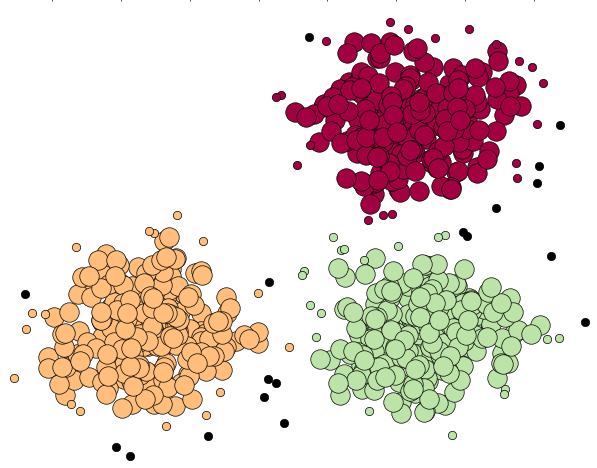
\includegraphics[scale = 0.55]{Cluster-Segmentation.png}
\end{flushright}

\begin{center}
\rule{\textwidth}{0.5pt}
\end{center}
\begin{multicols*}{2}
\noindent
\large Bruno Jácome, A89515\\
  Carolina Barros, A84950\\
  Dinis Gomes, A87993\\
  Joana Gouveia, A85650\columnbreak
  \\João Silva, A84617\\
  Jorge Gonçalves, A84133\\
  Pedro Peixoto, A89602
\end{multicols*}

%----------------------------------------------------------------------------------------
%	Índice
%----------------------------------------------------------------------------------------
\setlength{\leftmargini}{-0,35cm}
\setlength{\leftmarginii}{-0,35cm}
\setstretch{1.1}

\renewcommand*\contentsname{Índice}
\tableofcontents

\renewcommand{\listfigurename}{Lista de Figuras}
\listoffigures

\renewcommand{\listtablename}{Tabelas}


%----------------------------------------------------------------------------------------
%	ABSTRACT AND KEYWORDS
%----------------------------------------------------------------------------------------
\newpage

\setstretch{1.5}

\renewcommand{\chaptermark}[1]{\markboth{#1}{}}
\ifoot*{\color{gray}Universidade do Minho}
\ofoot*{\color{gray} \leftmark\hspace{0.25cm}|\hspace{0.25cm}\thepage}


%----------------------------------------------------------------------------------------
%	Introdução
%----------------------------------------------------------------------------------------
\chapter{Introdução}

Este trabalho foi realizado no âmbito da Unidade Curricular de Matemática das Coisas e teve como principal objetivo o estudo de clusters particionais com dados numéricos (centróide) através do  \textit{The Elbow Method}.\par
O presente relatório divide-se em 4 partes. Primeiramente, no Capítulo 2, será feita uma contextualização do assunto, apresentam-se a definição de clusters no geral e, mais em concreto, de clusters particionais.\par
Seguidamente, no Capítulo 3, será descrito o conceito de centróide, bem como outros aspetos relevantes associados a este conceito.\par
Depois, no Capítulo 4, serão abordados alguns algoritmos de clusters particionais, com a apresentação de algumas das suas aplicações mais práticas.\par
No capítulo seguinte, apresentar-se-á o \textbf{método de elbow}, o assunto principal deste trabalho.\par 
Para finalizar, expor-se-á uma breve conclusão do trabalho apontando-se essencialmente as desvantagens do método de \textit{elbow}.

%----------------------------------------------------------------------------------------
%	Definição de clusters 
%----------------------------------------------------------------------------------------
\newpage

\chapter{Clusters}
\section{O que são?}
\begin{wrapfigure}{r}{0.45\textwidth}
\vspace{-1cm}
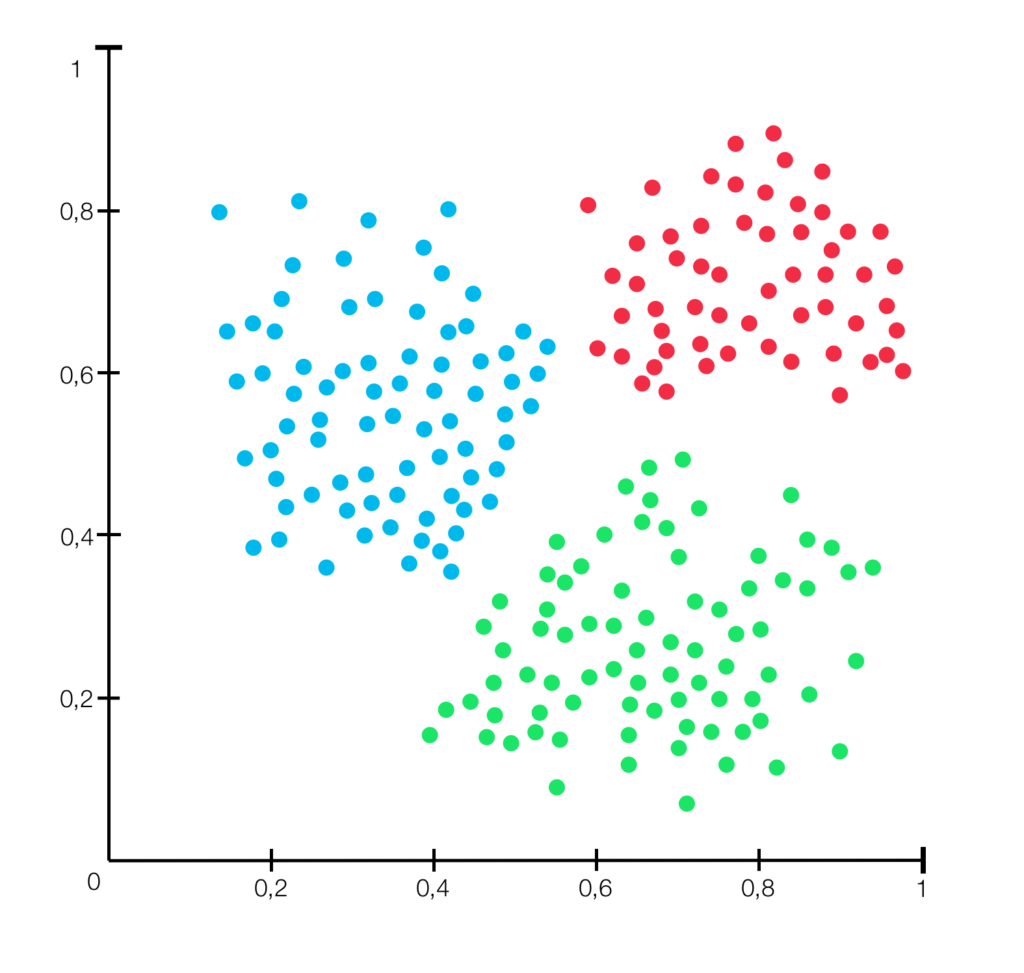
\includegraphics[scale=0.2]{cluster1.png}
\caption{Agrupamento de clusters.}
\end{wrapfigure}

\quad Um \textbf{cluster} é um conjunto de objetos similares entre si e dissimilares em relação a objetos noutros clusters. A análise de clusters ou o seu conceito, é um procedimento humano normal, muitas vezes usado de forma inconsciente.

\par A análise de clusters, é usada em inúmeras aplicações, tais como no reconhecimento de padrões (\textit{machine learning}), processamento de imagem e pesquisas de mercado \cite{clusterizacao, clustering}.



\section{Clusters Particionais}
\subsection{O que são?}
\quad Cluster particional define-se, especificamente, quando se utiliza um agrupamento que consiste em dividir os dados em subconjuntos sem que haja interseções, o que leva a que cada objeto esteja exatamente num subconjunto. Chamamos a estes subconjuntos uma partição dos dados.


\section{\textit{Clustering}}
\quad O \textit{clustering} é o conjunto de técnicas de prospeção de dados, isto é, exames minuciosos e metódicos que fazem agrupamentos automáticos de dados segundo o seu grau de semelhança. Normalmente o usuário do sistema deve escolher a priori o número de grupos a serem detetados. Alguns algoritmos mais sofisticados pedem apenas o número mínimo e outros tem a capacidade de subdividir um grupo em dois.


%---------------------------------------------------------
% Centróides
%---------------------------------------------------------


\chapter{Centróides}
\section{O que são?}
\quad Um \textbf{centróide} é o ponto que representa o \textit{centro} de todos os pontos pertencentes a um cluster.
No que diz respeito aos modelos centróides, a noção de similaridade está associada à proximidade dos pontos ao centróide do \textit{cluster}.\par
\par Os centróides são obtidos através de operações algébricas e, em regra, não pertencem à base de dados. Logo, são uma mera interpretação de resultados e dependem maioritariamente da definição de proximidade entre dois objetos de estudo.

\section{Relação entre centróide e média}
\subsection{Semelhanças}
\quad A \textit{média} de um cluster pode ser o centróide, contudo o termo \textbf{centróide} é mais preciso quando se estuda \textit{multivariate data}, isto é, dados multivariados. 
\par Um centróide é às vezes denominado de \textbf{centro de massa} ou  \textbf{barycenter} (centro de gravidade), baseado na sua interpretação física. Assim como a média, a localização do centróide \textbf{minimiza a soma dos quadrados das distâncias entre os pontos} ou \textbf{WCSS (With-in cluster sum-squared)}.



\subsection{Diferenças}
\par Há, no entanto, uma diferença entre \textbf{distância de centróide} e \textbf{distância média} quando se comparam clusters. A distância de centróide entre dois quaisquer clusters A e B é simplesmente a distância entre o centróide de A e o centróide de B. Já a distância média é calculada para cada cluster e é a média das distâncias entre todos os pontos do cluster e o centróide.

%------------------------------------------------------------
%	Algoritmos
%-----------------------------------------------------------

\chapter{Algoritmos de Clusters Particionais}
O Cluster Particional tem dois algoritmos: o \textit{K-means} e o \textit{K-medoids}. Estes algoritmos podem ser representados graficamente por diagramas de Voronoi criando \textbf{células de Voronoi}, que no caso do \textit{k-means}, cria células distintas associadas a cada centróide, isto é, distingue cada cluster. 


\section{K-means}
\subsection{O que é?}
\begin{wrapfigure}[8]{r}{0.5\textwidth}
  \centering
  \vspace{-2cm}
  \animategraphics[autoplay, loop, scale=0.8]{1}{kmeans/kmeans-}{0}{14} %14
  \caption{\normalfont Convergência do \textit{K-means}}
  \end{wrapfigure}
  
\quad O \textit{k-means} é um algoritmo iterativo de \textit{clustering} bastante comum e popular usado por numerosos investigadores em todo o mundo. Este tem por objetivo distribuir $m$ observações (totalidade dos \textit{data points}) por $k$ clusters, onde cada observação está dentro do cluster com o qual está mais próxima, usando o diagrama de \textit{Voronoi}.
Nestes modelos, os números de clusters necessários no final ($k$) têm de ser mencionados com antecedência, o que torna importante o conhecimento prévio do conjunto de dados. \cite{kmeans}
\vspace{-0.5cm}
\subsection{Restrições}
\quad Uma restrição que este algoritmo tem é o facto de apenas funcionar com atributos quantitativos, uma vez que requer operações algébricas, como somas e multiplicações por um escalar, o que dará origem a uma matriz que é chamada "matriz da partição". A nível de pontos que se encontram fora da curva representativa dos dados, terá de haver preocupação com os mesmo por puderem facilmente alterar o valor da média. 
\subsection{Algoritmo \textit{K-means}}

\begin{algorithm}
\caption{Pseudocódigo K-means}\label{kmeans}
\begin{algorithmic}
\Procedure{k-means}{K, conjunto de dados = \{$x^{(1)}, x^{(2)}, ..., x^{(m)}$\}}
\State Inicializar \textbf{aleatoriamente} K centróides $\mu_1, \mu_2, ..., \mu_K \in \mathbb{R}$
\Repeat
	\For {$i=1$ até $m$} \color{uminho}\Comment{\small Passo de associação de centróides\color{black}}
	\State$c^{(i)} := $ indíce (de $1$ até $K$) do centróide mais próximo de $x^{(i)}$ \color{uminho!70!black}\Comment{\small (dist($x^{(i)}$, $\mu_k$) mínima)\color{black}} 
	\EndFor
	\For {$k=1$ até $K$} \color{uminho}\Comment{\small Passo de reajustamento de centróides\color{black}}
	\State $\mu_k := $ ponto médio dos pontos no cluster $k$
	\EndFor
\Until{nenhum centróide se reajustar}

\EndProcedure
\end{algorithmic}
\end{algorithm}
\textbf{Nota:} Uma outra possibilidade para a inicialização dos $K$ centróides é escolhermos os primeiros $K$ elementos do conjunto dos dados $\left\{x^{(1)}, x^{(2)},\ldots, x^{(m)}\right\}$.

\medskip


\par Para $x^{(i)}=\left(x_1^{(i)}, \ldots,x_n^{(i)}\right)$ e $\mu_k=\left(\mu_1^{(k)},\ldots,\mu_n^{(k)}\right)$, temos
\begin{align*}
\dist(x^{(i)}, \mu_k)&=\|x^{(i)}-\mu_k\|\\
&=\sqrt{\left(x_1^{(i)}-\mu_1^{(k)}\right)^2+\cdots+\left(x_n^{(i)}-\mu_n^{(k)}\right)^2}.
\end{align*}
\par Minimizar $\|x^{(i)}-\mu_k\|$ equivale a minimizar $\|x^{(i)}-\mu_k\|^2$, ou seja, a determinar o mínimo da soma dos quadrados,
\[
 \|x^{(i)}-\mu_k\|^2=\left(x_1^{(i)}-\mu_1^{(k)}\right)^2+\cdots+\left(x_n^{(i)}-\mu_n^{(k)}\right)^2.
\]
\par Portanto, em vez de determinarmos o mínimo das distâncias $\dist(x^{(i)}, \mu_k)$, para $k=1, \ldots, K$, determinamos o mínimo dos quadrados das distâncias. Assim, se $c^{(i)}$ é o índice do centróide mais próximo de $x^{(i)}$, temos 
\[
\dist^2(x^{(i)}, \mu_{c^{(i)}})=\min_{k=1,\ldots, K}\|x^{(i)}-\mu_k\|^2.
\]

\par No final de cada iteração, os centróides são atualizados e cada novo centróide passa a ser o ponto médio dos pontos do respetivo cluster. O processo repete-se até que todos os clusters se mantenham inalterados. Ver pormenores em \cite{coursera1}.

\begin{figure}[h!]
  \begin{center}
  \animategraphics[controls, autoplay, loop, scale = 0.7]{24}{k2/kmeans-}{0}{898} %898
  \end{center}
  \caption{\normalfont\textit{k-means clustering} com \textbf{k = 2}}
\end{figure}


\newpage
\section{K-medoids}
\subsection{O que é?}
\begin{wrapfigure}[7]{r}{0.5\textwidth}
  \centering
  \vspace{-2cm}
  \animategraphics[autoplay, loop, scale=0.6]{1}{pam/pam-}{0}{6} %6
  \caption{\normalfont\textit{PAM} com \textbf{k = 3}}
  \end{wrapfigure}
O \textit{k-medoid} ou \textit{partitioning around medoids} (\textbf{PAM}) são algoritmos de \textit{clustering} reminiscentes do algoritmo de\break \textit{k-means}, na medida em que ambos operam de modo particional e ambos tentam minimizar a distância entre os pontos e o centróide, dentro de um cluster \cite{pam}.



\subsection{Medóide} 
\quad Uma ideia semelhante à de centróide é a de \textbf{medóide}, que é o \textit{data point} que é o \textit{menos parecido} de todos os outros \textit{data points}. 
\par Ao contrário do centróide, a medóide tem de ser um dos pontos originais. 



\section{Diferença entre K-means e K-medoids}
\quad A nível de sensibilidade, o \textit{K-medoid} lida melhor com os \textit{outliers} (pontos fora da curva) do que o \textit{K-means}. É menos sensível a eles, porque minimiza a soma das diferenças, contrariamente a \textit{k-means}, que maximiza.
\par No que diz respeito ao centróide, o centro de \textit{k-medoids} não é o ponto médio mas sim um ponto real, porque é o objeto mais centralmente localizado do cluster, que como já referimos, tem somas mínimas de distância.
\par Quanto aos atributos, os atributos de \textit{K-medoids} podem ser quantitativos, tal como \textit{k-mean}, mas também podem ser qualitativos, o que leva a que não exista uma necessidade e obrigação do uso de operações algébricas neste algoritmo. Estes atributos encontram-se representados na base de dados.


%----------------------------------------------------------------------------------------
%"The Elbow Method"
%----------------------------------------------------------------------------------------

\chapter{O Método de \textit{Elbow}}
\section{O que é?}
\quad Uma etapa fundamental para qualquer aprendizagem não-supervisionada é determinar o número ideal de clusters nos quais os dados podem ser agrupados: \textbf{K}.
\par O \textbf{Método de Elbow} é uma heurística, uma vez que é um método criado para encontrar soluções sobre um problema complexo, como uma medida que preserva e conserva energia e os recursos mentais. Neste caso, para determinar o número ideal de clusters no \textit{k-means clustering}, este método parcela o valor da função custo produzida pelos diferentes valores de \textbf{K}. Ora, isto só é possível ignorando parte da informação com o objetivo de tornar a escolha mais fácil e rápida.
\par
Sendo assim, não há uma resposta universal para este problema já que o número ideal de clusters é de alguma forma subjetivo e depende não só do propósito do \textit{clustering}, mas também do método usado para medir as similaridades e os parâmetros usados para particionar. 

\begin{figure}[h!]
\centering
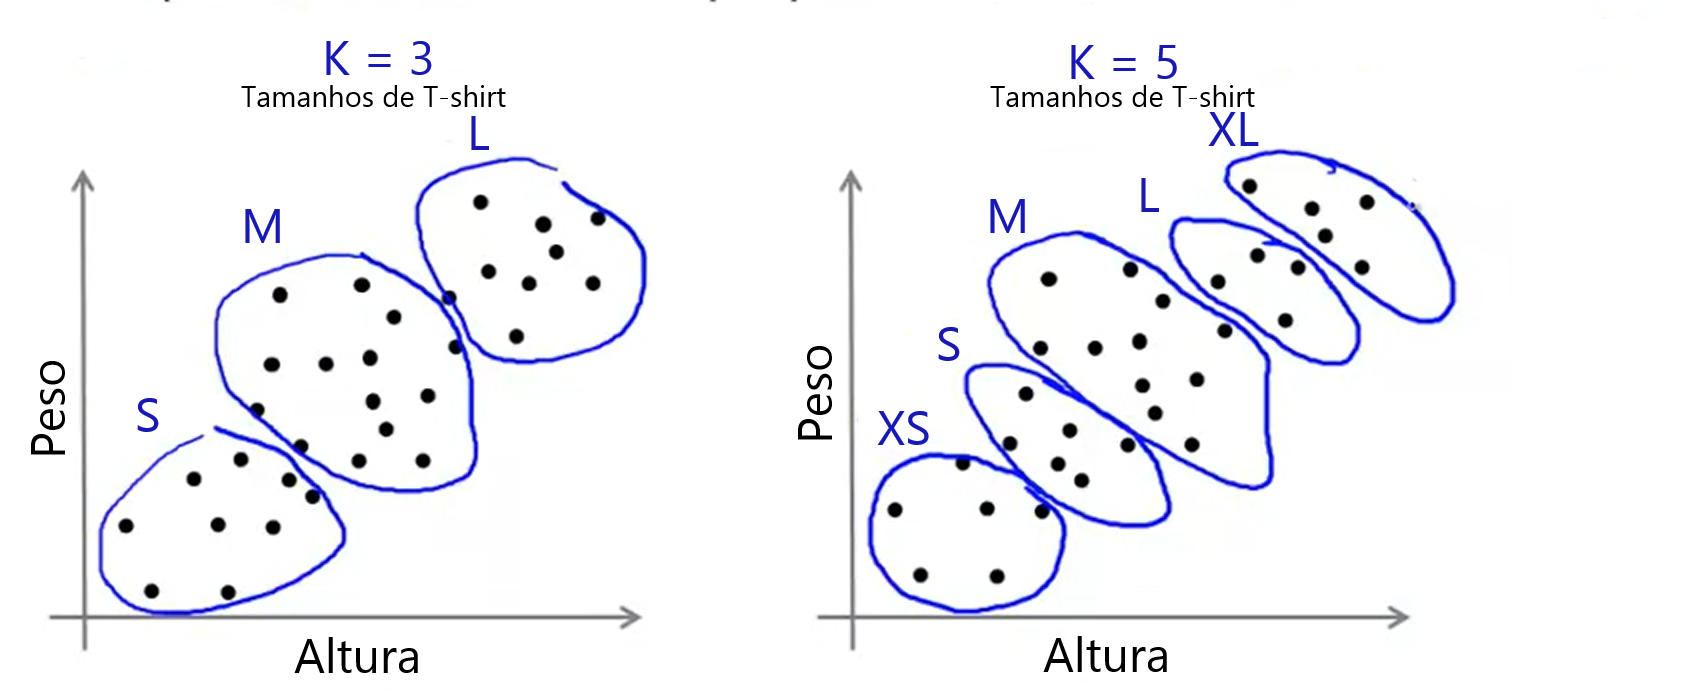
\includegraphics[scale=0.3]{example_clustering1}
\caption{Número de clusters (3 \textit{vs} 5) representando tamanhos de \textit{t-shirts}.}
\end{figure}
Ver mais detalhes em \cite{coursera2}.
\newpage
\section{Pré-aplicação}
\quad
Numa fase inicial, é útil criar um dendrograma, isto é, um diagrama que organize as variáveis, agrupando-as de forma hierárquica ascendente - o que em termos gráficos se assemelha aos ramos de uma árvore.
\par 
Seguidamente, deve-se inspecionar o dendrograma produzido usando o cluster hierárquico para verificar se este sugere um número específico de clusters. Todavia, esta abordagem também é subjetiva.
\par
Estes métodos incluem métodos diretos e de teste estatístico.
\begin{itemize}[leftmargin=1cm]
\item \textbf{Métodos diretos}: consistem em otimizar um critério, como a somas dos quadrados das distâncias dentro dos clusterss. (\textit{WCSS - With-in Cluster Sum of Squares}) ou a média \textit{silhouette}. Os métodos correspondentes são denominados métodos de \textit{Elbow} e \textit{silhouette}, respetivamente.
\item \textbf{Métodos de teste estatístico}: consistem em comparar evidências contra hipóteses nulas. Um exemplo é a estatística de \textit{gap}.
\end{itemize}
%----------------------------------------------------------------------------------------
\section{WCSS}

\subsection{Ilusão de solução ótima}

\begin{wrapfigure}{r}{0.5\textwidth}
  \centering
  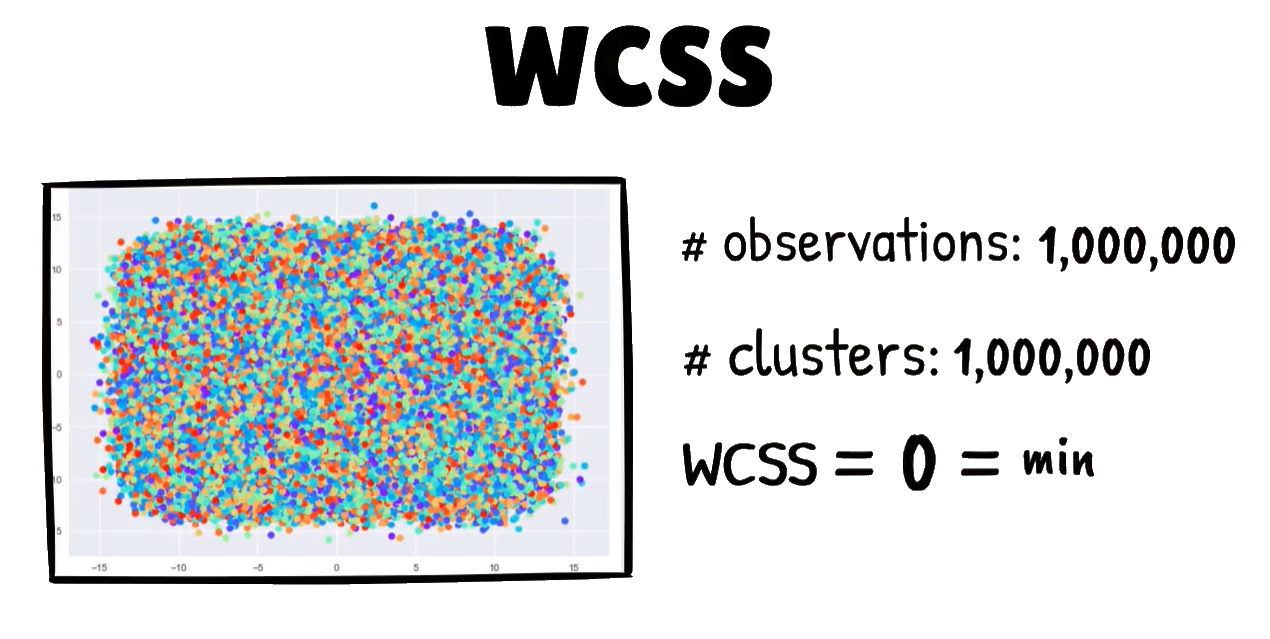
\includegraphics[scale=0.25]{wcss_global_minimize}
  \caption{\textit{WCSS} mínimo}
  \label{fig:wcss_min}
\end{wrapfigure}
  
\par Comummente, considera-se que para se obter a solução ótima de número de clusters, deve-se calcular o mínimo de \textbf{WCSS}. 
Porque será então isto um erro?

\par Para um valor mínimo de \textit{WCSS}, a solução ótima de número de clusters é igual ao número total de \textit{data points}. A noção de cluster acaba por perder o seu propósito, pois temos uma solução trivial para o problema.


\begin{wrapfigure}[6]{l}{0.5\textwidth}
  \centering
  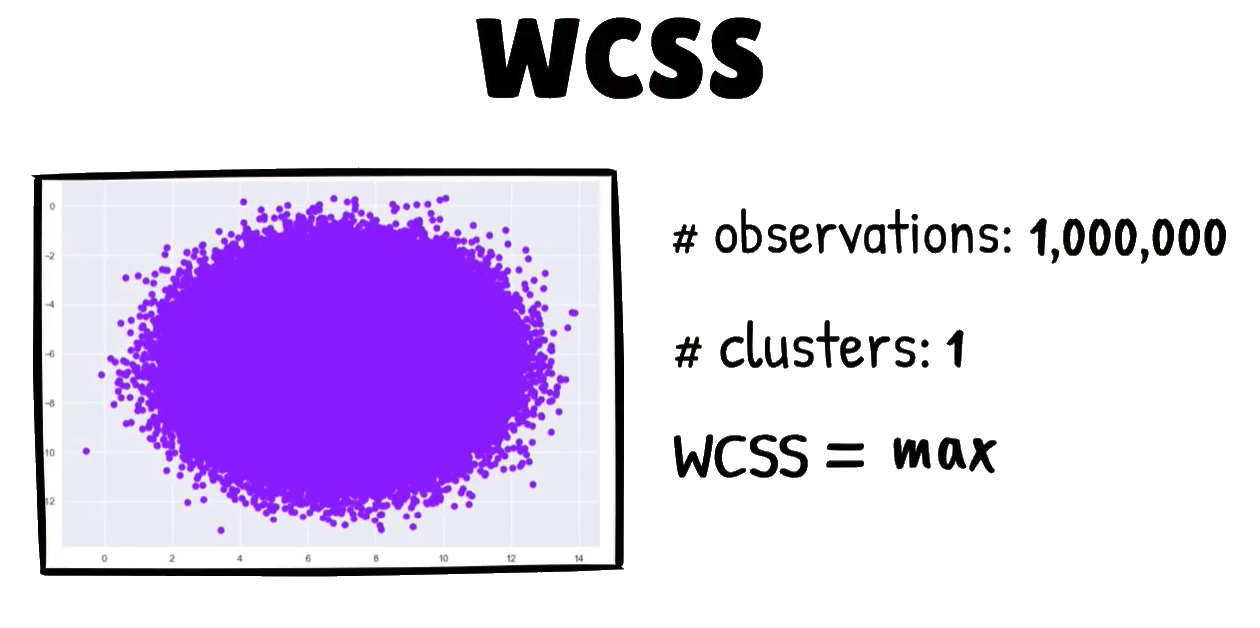
\includegraphics[scale=0.25]{wcss_maximize}
  \caption{\textit{WCSS} máximo}
\end{wrapfigure}

\par Por oposição, para um valor máximo de \textit{WCSS}, a solução ótima seria apenas um cluster. Isto é óbvio uma vez que a soma dos quadrados das distâncias \textit{intra-cluster} só poderia ser máxima se este contivesse todos os pontos.

\subsection{Solução ótima para o problema}

\begin{wrapfigure}[7]{r}{0.4\textwidth}
  \centering
  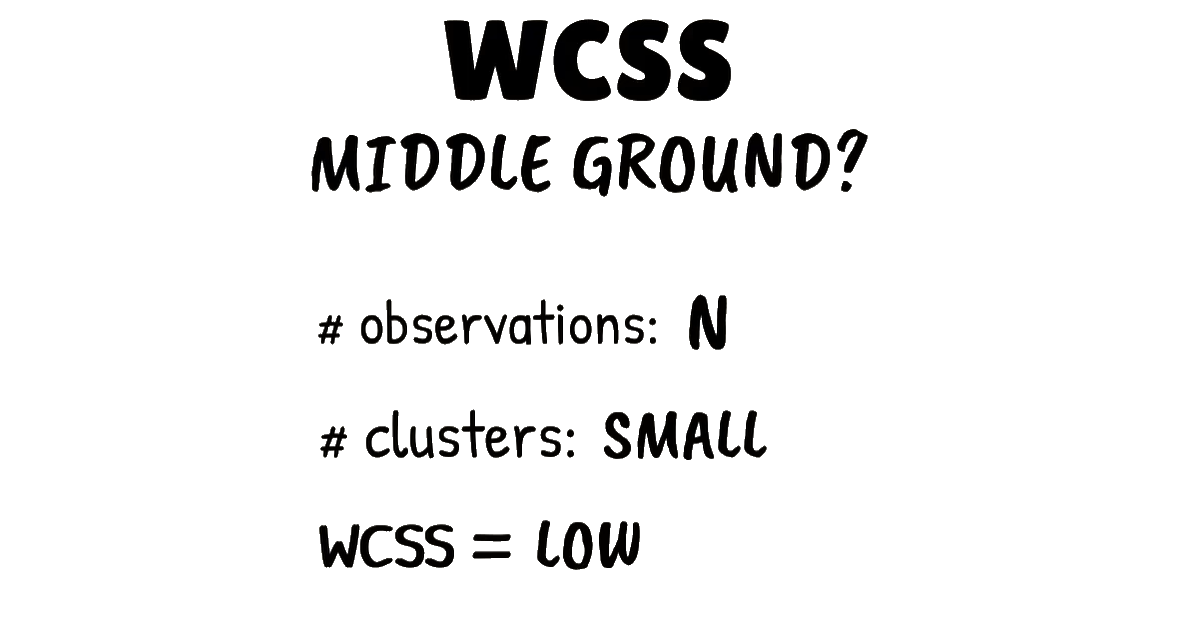
\includegraphics[scale=0.25]{wcss_otimo}
  \caption{Solução ótima}
  \end{wrapfigure}
  
\quad Em boa verdade, não há uma solução ótima.
Como foi dito anteriormente, o número de clusters ótimo depende de vários fatores, inclusivé do objetivo de cada "clusterização"\space específica. 


\par Contudo, com a ajuda do \textbf{método de Elbow}, é possível obter um resultado ótimo de \textbf{equilíbrio} entre o \textbf{número de clusters} e \textbf{WCSS}.



%--------------------------------------------------
\section{Aplicação}
\quad O método de Elbow considera o \textit{WCSS} total como uma função do número de clusters: deve-se escolher um número de clusters para que a adição de outro cluster não melhore muito mais o \textit{WCSS} total. Ver \cite{Yellowbrick, datanovia}.
\par O número ótimo de clusters pode ser obtido da seguinte forma:\par
\begin{enumerate}[leftmargin=2cm, align=left]
\item	Aplicar o algoritmo de \textit{clustering}, por exemplo, \textit{k-means clustering}, para diferentes valores de \textit{k}.
\item	Para cada \textit{k}, calcular o \textit{WCSS}.
\item	Representar, graficamente, o \textit{WCSS} em função do k.
\item	Localizar, no gráfico, a curva com uma aparência de \textbf{cotovelo (elbow)}, geralmente considerado o indicador do número ótimo de \textit{clusters}.
\end{enumerate}



\begin{figure}[h]
  \begin{center}
  \animategraphics[controls, autoplay, loop, scale = 0.65]{24}{elbow_method/elbow-}{0}{956} %956
  \end{center}
  \caption{\normalfont Procedimentos do método de \textit{elbow}}
  \end{figure}


\begin{figure}[h!]
  %\begin{wrapfigure}{r}{0.6\textwidth}
    \centering
    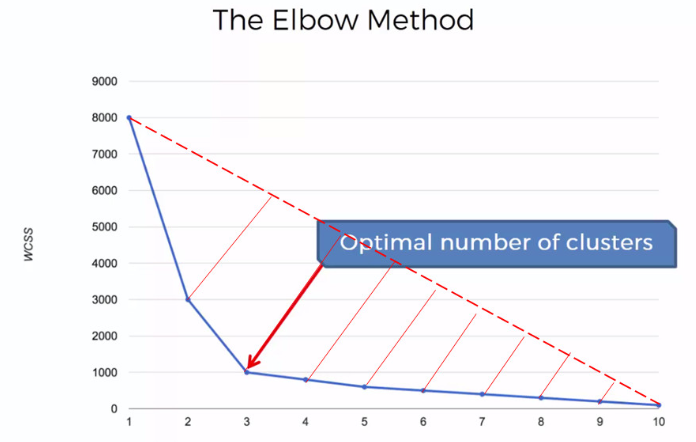
\includegraphics[scale=0.6]{3.png}
    \caption{Valor de WCSS \textit{versus} número de \textit{clusters}}   
    \label{wrapfig:wcss_k}
 % \end{wrapfigure}
\end{figure}

\textsc{Asanka Perera}\cite{asanka} afirma que, "após ter lido alguns artigos, descobriu que se desenharmos uma
linha reta entre o ponto 1 e 10, e se calcularmos a distância de cada ponto até à linha, o ponto com
a maior distância será o ponto que contém o cotovelo".


%-------------------------------------------------------
% Conclusão
%-------------------------------------------------------

\chapter{Conclusões}

\indent O método de \textit{Elbow}, apesar de bastante prático por ser um método visual, tem uma interpretação subjetiva e nem sempre muito clara.
Mais concretamente, o verdadeiro \textit{elbow}(cotovelo), nem sempre é identificado sem ambiguidade, já que pode acontecer não haver nenhum \textit{elbow} ou haver mais do que um. 
\par Além disso, verifica-se, em geral, que ocorrem descidas abruptas no \textit{WCSS} até k=3 e a partir deste valor a curva desce lentamente. De facto, como é explicado na figura \ref{fig:wcss_min}, à medida que K cresce, o número de \textit{data points} por cluster diminui, e o \textit{WCSS} também. Quando K é igual ao número total de \textit{data points}, o \textit{WCSS} é 0. Logo, torna-se óbvio que o número ideal de clusters nunca deverá ser elevado, a menos que o utilizador o queira, mas nesse caso nem fará sentido à aplicação método.
\par Outros problemas associados ao método de \textit{elbow}, devem-se à aplicação do algoritmo de \textit{clustering} \textit{k-means}. O procedimento mais comum usa uma técnica de refinamento iterativo e é muitas vezes chamado de algoritmo de \textit{Lloyd}. Embora existam alternativas bem mais eficientes, este algoritmo tem um longo tempo de execução, particularmente devido ao cálculo das distâncias de cada ponto aos K centróides. A maior parte dos pontos ficam associados aos mesmos centróides após algumas iterações e, por isso, a maior parte deste trabalho é inútil, tornando esta implementação bastante ineficiente. 
\par Apesar das dificuldades referidas, que aparecem sobretudo quando o número de \textit{data points} é \textit{elevado}, a aplicação do método de \textit{elbow} em combinação com o \textit{k-means} produz resultados bastante satisfatórios em diversas aplicações.  





\pagestyle{empty}
\begin{thebibliography}{9}
\clearpairofpagestyles


\bibitem{Yellowbrick}
\textsc{The scikit-yb developers},
{\em Elbow Method},
\\\url{https://www.scikit-yb.org/en/latest/api/cluster/elbow.html}
\\(13/04/2020)


\bibitem{datanovia}
{\em Determining The Optimal Number Of Clusters: 3 Must Know Methods},
\\\url{https://www.datanovia.com/en/lessons/determining-the-optimal-
number-of-clusters-3-must-know-methods/\#elbow-method}
\\(13/04/2020)


\bibitem{asanka} 
\textsc{Asanka Perera},
{\em Finding the optimal number of clusters for K-Means through Elbow
method using a mathematical approach compared to graphical approach},
\\\url{https://www.linkedin.com/pulse/finding-optimal-number-clusters-k-means-through-
elbow-asanka-perera}
\\(13/04/2020)


\bibitem{Lachi} 
\textsc{Lachi, Ricardo Luís \& Rocha, Heloísa Vieira da. Fevereiro 2005},
{\em Aspectos básicos de \textit{clustering}: conceitos e técnicas(Brasil)}
\\(13/04/2020)


\bibitem{clusterizacao}
\textsc{Rodrigo Cezar Menezes},
{\em Clusterização de Dados},
\\\url{https://www.maxwell.vrac.puc-rio.br/24787/24787_5.PDF}
\\(13/04/2020)


\bibitem{clustering}
\textsc{Manuel Altino Torres Aniceto Castro},
{\em Agrupamento – “Clustering”},
\\\url{http://www.dei.isep.ipp.pt/~paf/proj/Julho2003/Clustering.pdf}
\\(13/04/2020)



\bibitem{dist_clusters}
\textsc{Victor Lavrenko},
{\em Hierarchical Clustering 3: single-link vs. complete-link},
\\\url{https://www.youtube.com/watch?v=VMyXc3SiEqs}
\\(13/04/2020)




\bibitem{kmeans-clustering}
\textsc{Victor Lavrenko}
{\em K Means Clustering: Pros and Cons of K Means Clustering},
\\\url{https://www.youtube.com/watch?v=YIGtalP1mv0}
\\(13/04/2020)



\bibitem{elbow_method}
\textsc{Test My ChatBot},
{\em How to Choose the Number of Clusters | Advanced Statistical Methods - K-Means Clustering},
\\\url{https://www.youtube.com/watch?v=SCA07-7Xe6Q}
\\(13/04/2020)



\bibitem{pam}
{\em k-medoids},
\\\url{https://en.wikipedia.org/wiki/K-medoids}
\\(13/04/2020)

\bibitem{coursera1}
\textsc{Universidade de Stanford},
{\em K-Means Algorithm},
\\\url{https://pt.coursera.org/lecture/machine-learning/k-means-algorithm-93VPG}
\\(13/04/2020)


\bibitem{coursera2}
\textsc{Universidade de Stanford},
{\em K-Means Algorithm},
\\\url{https://pt.coursera.org/lecture/machine-learning/choosing-the-number-of-clusters-Ks0E9}
\\(13/04/2020)

\bibitem{kmeans}
{\em k-means clustering},
\\\url{https://en.wikipedia.org/wiki/K-means_clustering}
\\(13/04/2020)

\end{thebibliography}

\end{document}